\chapter{Teori}\label{Teori}

\section{Brystets opbygning og brystkræft}
Bryster er sammensat af mange små brystkirtler, bestående af kirtelceller til producering af mælk, og udførselsgange, som samler sig frem til brystvorten. Mænds bryst er opbygget ligesom kvindebrystet, dog uden fungerende mælkekirtler \cite{Mand}. Brystkirtlerne er omgivet af fedt og bindevæv\citep{Bryst}.

\begin{figure}[H]
    \centering
    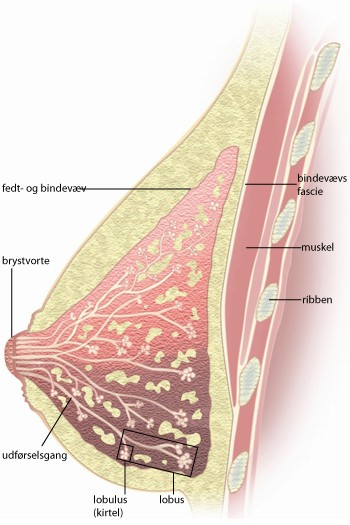
\includegraphics[width=0.35\textwidth]{figurer/r/bryst}
    \caption{Brystets opbygning \citep{Bryst}}
    \label{Brystet}
\end{figure}

I brystet kan der opstå brystkræft, hvor det hyppigst opstår i en udførselsgang \citep{Bryst}. Brystkræft er den mest udbredte kræftform hos kvinder, men den kan også opstå ved mænd. Det er dog meget hyppigere hos kvinder \cite{Mand}.

Forstadiet til brystkræften sker ved en mutation af cellernes gener. Denne mutation kan ske over tid, men kan også være et arvet gen. Mutationen gør, at cellerne ændrer form og udseende, da cellerne deler sig for meget, hvilket danner en knude. Normalt vil syge celler nedbrydes, men dette sker ikke ved kræftceller, som hele tiden deler sig og skaber nye kræftceller. Bliver udviklingen af kræftcellerne ikke behandlet, vil kræftcellerne med tiden brede sig til det omkringliggende væv \cite{Udvikling}. 

\section{Ultralydsscanning}
Ultralyd er højfrekvent lyd, hvor man til ultralydsscanning benytter frekvenser mellem 2 og 20 MHz \cite{Frekvens}. Der anvendes en ultralydsprobe, som er en transducer. Transduceren indeholder piezoelektriske krystaller, som skaber lydbølger, når de bliver udsat for en elektrisk spænding. Disse lydbølger udsendes mange gange i sekundet fra transduceren og reflekteres tilbage til transduceren, når de møder væv. Ud fra lydbølgerne, transduceren modtager, dannes en ultralydsscanning, som lægen kan diagnosticere ud fra \cite{Ultralydsscanning}.

På ultralydsscanningen ses kirtelvæv som lyse områder, mens kræftknuder fremtræder som mørke skygger. Der er derfor en god kontrast mellem kirtelvæv og kræftknude på et ultralydsbillede \cite{Ultralyd}.

\section{Røntgenundersøgelse}
Røntgenstråler er elektromagnetiske bølger med en kortere bølgelængde end synligt lys. Strålerne er ioniserede, og derfor er det vigtigt at give den korrekte dosis, der måles med enheden milliSievert (mSv). Ved mammografiscanninger med røntgen benyttes en dosis på 0,5 mSv. \cite{Sundhedsstyrelsen}. Livstidsrisikoen for at inducere kræft efter en mammografiscanning med røntgen er definieret som meget lille, hvilket betyder, at 1 ud af 100.000 til 1 ud af 10.000 rammes \cite{Risk}. 

Ved røntgenundersøgelser sendes røntgenstrålerne fra et røntgenrør gennem patienten og opfanges på en fotografisk film, som vil danne billedet alt afhængig af, hvor meget af strålingen, der bliver absorberet i kroppen \cite{Rontgenundersogelse}.

På røntgenbilleder ses fedt og andre bløddele som grå skygger, da de ikke absorberer så mange røntgenstråler, hvorimod kræftknuder absorberer meget røntgenstråling og derfor ses som lyse områder \cite{Rontgenundersogelse}.

På billedet \ref{rontgen} nedenfor ses et røntgenbillede af brystvæv. Kræftknuden ses tydeligt som den lysende plet, markeret med en firkant. Figur \ref{teo} nedenfor viser en tegning af hvad der ses på figur \ref{ultralyd}. Billedet \ref{ultralyd} viser et stilbillede af en ultralydsscanning af brystvæv. På billedet ses kræftknuden som en mørk skygge. 

\begin{figure}[H]
  \centering
    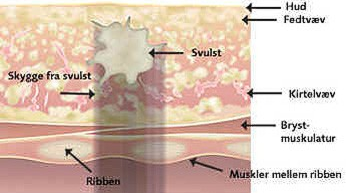
\includegraphics[width=\textwidth]{figurer/r/teori}
    \caption{Teoretisk tegning af hvad der ses på billedet ovenfor \cite{Ultralyd}}
    \label{teo}
\end{figure}

\begin{figure}[H]
  \centering
  \begin{minipage}{0.4\textwidth}
    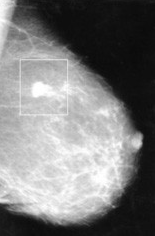
\includegraphics[width=\textwidth]{figurer/r/rontgen}
    \caption{Røntgenbillede af brystvæv \cite{Mammografi}}
    \label{rontgen}
  \end{minipage}
  \hfill
  \begin{minipage}{0.4\textwidth}
    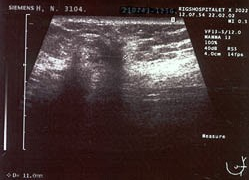
\includegraphics[width=\textwidth]{figurer/r/ultra}
    \caption{Ultralydsbillede af brystvæv \cite{Ultralyd}}
    \label{ultralyd}
  \end{minipage}
\end{figure}

